\documentclass{scrartcl}

\usepackage{german}
\usepackage[utf8]{inputenc}  %Umlaute
\usepackage[T1]{fontenc}     %Umlauttrennung
\usepackage{lmodern}         %modernes Schriftbild
\usepackage{amsmath}         %math Umgebungen
\usepackage{graphicx}
\usepackage{hyperref}        %URLs
\usepackage{gensymb}         %Gradzeichen
\usepackage{float}           %Positionierung von Tabellen und Abb
\usepackage{textgreek}


\begin{document}
\begin{titlepage}
  \begin{center}
    \vspace*{1cm}
    \LARGE
    Physikpraktikum für Naturwissenschaftler \\
    \vspace*{1cm}
    \Huge
    \textbf{Versuch: Viskosität} \\
    \vspace*{0.3cm}
    \Large
    Durchgeführt am 17. Januar 2019 \\
    Betreuer: Florian Nägele \\
    \vspace*{2.5cm}
    Gruppe 13 \\
    Felix Burr: felix.burr@uni-ulm.de \\
    Johannes Spindler: johannes.spindler@uni-ulm.de \\
    \vfill 
  \end{center}
  Wir bestätigen hiermit, das Protokoll selbstständig erarbeitet zu haben und in genauer Kenntnis über dessen Inhalt zu sein. \\
  \vspace*{0.8cm}
  \\
  Felix Burr
  \hfill
  Johannes Spindler
\end{titlepage}
\pagebreak
\tableofcontents


\pagebreak

\section{Einleitung}





\section{Bestimmung der Viskosität von Getriebeöl mit der Kugelfallmethode}
\subsection{Versuchsaufbau und Durchführung}
\subsection{Messwerte und Ergebnisse}
\begin{table}[H]
\captionof{table}{Messwerte für die Kugeldurchmesser d\textsubscript{i}}
\begin{center}
\begin{tabular}{l|l|l|l|l}
Messung   &   d\textsubscript{1} [mm]   &   d\textsubscript{2} [mm]   &   d\textsubscript{3} [mm]   &   d\textsubscript{4} [mm] \\
\hline
1 & 0,99 & 2,00 & 2,99 & 3,99 \\
2 & 1,00 & 1,99 & 2,99 & 3,99 \\
3 & 1,00 & 1,99 & 2,99 & 3,99 \\
\hline
d [mm] & 1,00 & 1,99 & 2,99 & 3,99 \\
\textsigma(d) [mm] & 0,01 & 0,01 & 0,00 & 0,00 
\end{tabular}
\end{center}
\label{tab:Kugeldurchmesser}
\end{table}

\begin{table}[H]
\captionof{table}{Messwerte für die Fallzeiten t\textsubscript{i}}
\begin{center}
\begin{tabular}{l|l|l|l|l}
Messung   &   t\textsubscript{1} [s]   &   t\textsubscript{2} [s]   &   t\textsubscript{3} [s]   &   t\textsubscript{4} [s] \\
\hline
1 & 146 & 36 & 18,31 & 10,21 \\
2 & 143 & 37 & 16,25 & 10,38 \\
3 & 142 & 37 & 17,53 & 10,11 \\
4 & 142 & 37 & 17,00 & 10,56 \\
5 & 144 & 38 & 16,84 &  9,00 \\
6 & 145 & 37 & 17,12 & 10,02 \\
7 & 143 & 38 & 16,81 & 10,06 \\
8 & 144 & 37 & 16,75 &  9,68 \\
9 & 144 & 37 & 16,87 &  9,93 \\
10 & 143 & 37 & 16,81 & 10,75 \\
\hline
t [s] & 143,60 & 37,10 & 17,03 & 10,07 \\
\textsigma(d) [mm] & 1,26 & 0,57 & 0,55 & 0,49 
\end{tabular}
\end{center}
\label{tab:Fallzeiten}
\end{table}

\begin{table}[H]
\captionof{table}{Berechnete Viskositäten }
\begin{center}
\begin{tabular}{l|l|l|l|l}
Messung   &   1   &   2   &   3   &   4 \\
\hline
\texteta [mPa $cdot$ s] & 1789 & 1859 & 1919 & 2021 \\
2\textDelta d/d & 0,020 & 0,010 & 0,007 & 0,005 \\
\textDelta L/L & 0,003 & 0,003 & 0,003 & 0,003 \\
\textDelta t/t & 0,009 & 0,015 & 0,032 & 0,048 \\
\textDelta \texteta [mPa $cdot$ s] & 58 & 53 & 81 & 115
\end{tabular}
\end{center}
\label{tab:Viskositäten}
\end{table}
\subsection{Ergebnisdiskussion}





\section{Statistische Auswertung der Kugelfallmethode}
\subsection{Versuchsaufbau und Durchführung}
\subsection{Messwerte und Ergebnisse}
\begin{figure}[H]
  \centering
    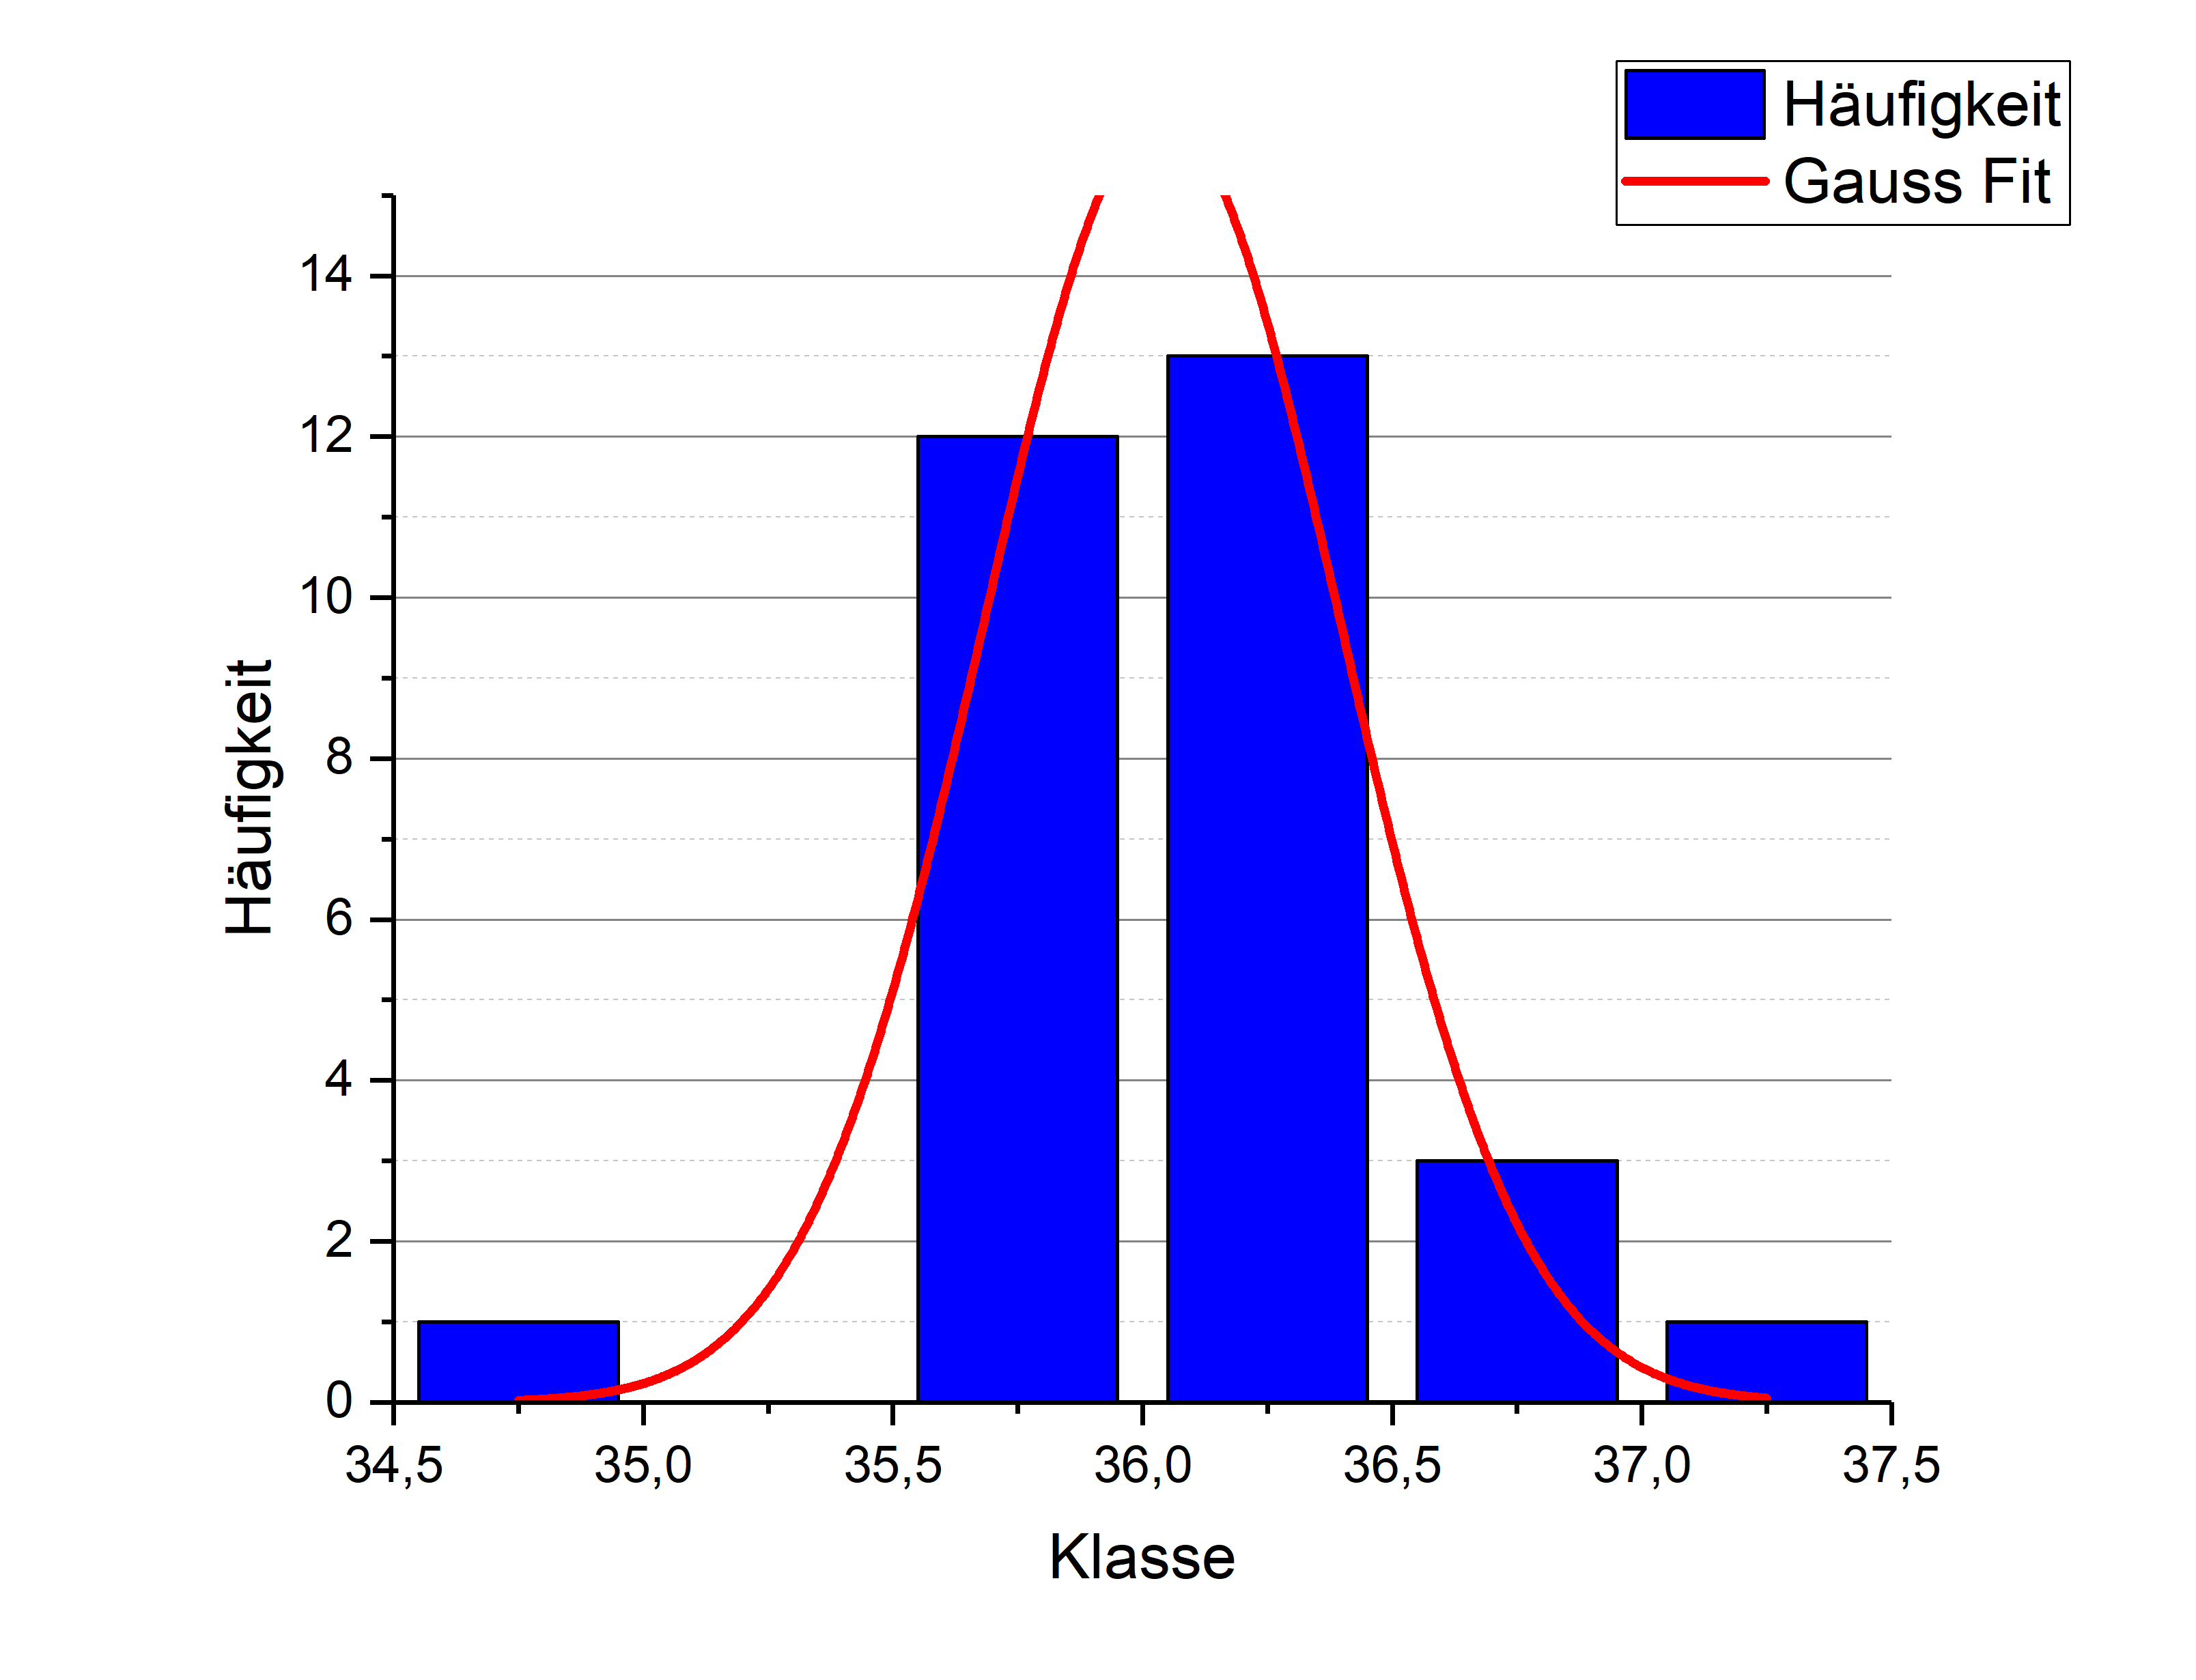
\includegraphics[scale=0.4]{GaussFit.PNG}
  \caption{Histogramm der Fallzeiten der 2-mm-Kugeln und daran angenäherte Normalverteilung)}
  \label{fig:GaussFit}
\end{figure}
\subsection{Ergebnisdiskussion}





\section{Bestimmung der Glycerinkonzentration mit dem Kapillarviskosimeter}
\subsection{Versuchsaufbau und Durchführung}
\subsection{Messwerte und Ergebnisse}
\subsection{Ergebnisdiskussion}
\end{document}